\section{Class 6 - 15/03/21}
\subsection*{Transmission line with general load $\bm{Z_0}$}
In the previous lectures we saw the transmission line in short circuit or open circuit, but those case are not the most common one, today we will see the most general situation when the load is a complex number $Z_L=a+jb$, like in \cref{fig:tl_with_general_load}.
\begin{figure}[H]
    \begin{center}
        \begin{circuitikz} 
            \draw (2,2)
            to[short, o-o] (7,2)
            to[short] (8.5,2)
            to[generic=$Z_{l}$] (8.5,0)
            to[short, -o](7,0)
            to[short, -o](2,0)
            ;
            \draw (4.5,0.45)node[label={[font=\LARGE]above:$Z_0$}] {}
            ;
          \end{circuitikz}     
    \end{center} \caption{Forward and backward wave signal in a TL}\label{fig:tl_with_general_load} 
\end{figure}
%We recall the voltage wave equation: $V\bottomPlus\,e^{\,j\beta l}+V\bottomMinus\,e^{\,-j\beta l}$.\\
% What we want for a great TL is to have only $V\bottomPlus$, or at least $V\bottomPlus > V\bottomMinus$
Now, what we want to do is to attempt some magic trick to modify the wave equation in \cref{eq:wave_solution_no_losses}, maybe we find a way to evaluate better how the reflected signal is affecting the line.
\begin{equation}
    V\bottomPlus =(V\bottomPlus - V\bottomMinus) + V\bottomMinus
\end{equation}
Then we can write the voltage over the line as:
\begin{align}
    \begin{split}
      V(l)&=\left[(V\bottomPlus - V\bottomMinus)+V\bottomMinus\right]e^{\,-j\beta l}+V\bottomMinus\,e^{\,j\beta l}=\\[5pt]
      &=(V\bottomPlus - V\bottomMinus)e^{\,-j\beta l}+V\bottomMinus\,e^{\,-j\beta l}+V\bottomMinus\,e^{\,j\beta l}=\\[5pt]
      &=(V\bottomPlus - V\bottomMinus)e^{\,-j\beta l}+V\bottomMinus\,\left(e^{\,-j\beta l}+e^{\,j\beta l}\right)=\\[5pt]
      &=(V\bottomPlus - V\bottomMinus)e^{\,-j\beta l}+2\,V\bottomMinus\,\cos(\beta l)
    \end{split}\label{eq:new_form_of_voltage_over_TL}
  \end{align}
  We skipped some passages, but that should only be the application of the trigonometric form of a complex number.\\
  We can notice from \cref{eq:new_form_of_voltage_over_TL} that the voltage over a TL is composed by two terms:
  \begin{itemize}
      \item $\bm{(V\bottomPlus - V\bottomMinus)e^{\,j\beta l}}$: This is the equation of a direct wave with amplitude $(V\bottomPlus - V\bottomMinus)$. The amplitude is not $V\bottomPlus$ because part of the wave is reflected backward
      \item $\bm{2\,V\bottomMinus\,\cos(\beta l)}$: This is the expression of a stationary wave. This part is "eating" part of the forward wave, this mean that if i fall in some "unlucky" point inside my TL the signal will be distorted.
  \end{itemize}

If i want to go back to the time domain with the forward wave using the usual formula in \cref{eq:from_phas_to_time_TL}:
\begin{equation}
    V(l,t)=(V\bottomPlus - V\bottomMinus)\cos(\omega t-\beta l)+2V\bottomMinus\cos(\omega t)\cos(\beta l)
\end{equation}
We find again a stationary wave (just as expected).
\subsection*{Module of the voltage wave in phasor}
Before to introduce the next topic (SWR), we need to introduce how we can calculate the module of the voltage wave in phasor domain.\\
In \cref{fig:voltage_components_in_phas} you can see the graphical representation of the two components that build up the voltage wave in complex domain that we have already seen in \cref{eq:current_and_voltage_in_TL_phas}.
\begin{figure}[H]    
    \begin{center}
        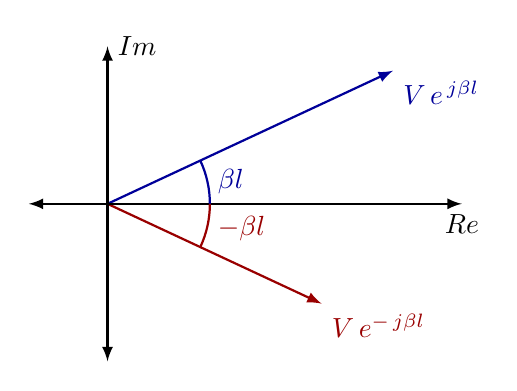
\begin{tikzpicture}[>=latex]
            \draw[style=help lines] (0,0) (3,2);
        
            \coordinate (vec1) at (-25:3); 
            \coordinate (vec2) at (25:4);
            \coordinate (vec3) at (0:4.5);
            \coordinate (vec4) at (90:2);
            \coordinate (vec5) at (270:2);
            \coordinate (vec6) at (180:1);
        
            \draw[->,thick,blue!60!black] (0,0) -- (vec2) node[below right] {$V\bottomMinus\,e^{\,j\beta l}$}; 
            \draw[->,thick,red!60!black] (0,0) -- (vec1) node[below right] {$V\bottomPlus\,e^{-\,j\beta l}$};
            \draw[->,thick,black] (0,0) -- (vec3) node [below] {$Re$};
            \draw[->,thick,black] (0,0) -- (vec4) node [right] {$Im$};
            \draw[->,thick,black] (0,0) -- (vec5);
            \draw[->,thick,black] (0,0) -- (vec6);
        
            \draw [blue!60!black, thick] (1.3,0) 
            arc [start angle=0, end angle=25, radius=1.3cm]
            node [midway, right] {$\beta l$}; 
            \draw [red!60!black, thick] (0:1.3) 
            arc [start angle=0, end angle=-25, radius=1.3cm]
                node [midway, right,yshift=-1] {$-\beta l$};
        \end{tikzpicture}
    \end{center}\caption{Forward and backward Voltage wave in phasor domain}\label{fig:voltage_components_in_phas}
\end{figure}
What we are doing now is to find a proper way to describe the module of $\phas{V}(l)$, that is NOT the real voltage value in the TL (remember that we are in phasor domain).\\
If you remember how we defined $\rho$\footnote{remember that $\rho$ and $\rho_L$ are the same thing with different name} in \cref{eq:reflection_coeff_at_load}, there is no doubt that we can write:
\begin{equation*}
    \rho= \frac{V\bottomMinus}{V\bottomPlus}
\end{equation*}
So the voltage equation in \cref{fig:voltage_components_in_phas} will become:
\begin{align}
    \begin{split}
        \phas{V}(l) &= V\bottomPlus \,e^{\,-j\beta l}+\rho\, V\bottomPlus \,e^{\,j\beta l}=\\[5pt]
        &= V\bottomPlus \left(e^{\,-j\beta l}+\rho \, e^{\,j\beta l}\right)
    \end{split}
\end{align}
Now, the best way to compute the module is to obtain it from $|\phas{V}(l)|^2$:
\begin{align}
    \begin{split}
        |\phas{V}(l)|^2 &= \phas{V}(l)\,\phas{V}^*(l) =\\[5pt]
        &=|V\bottomPlus|^2\,\left(e^{\,-j\beta l}+\rho \, e^{\,j\beta l}\right)\,\left(e^{\,-j\beta l}+\rho \, e^{\,j\beta l}\right)^*=\\[5pt]
        &= |V\bottomPlus|^2\,\left(e^{\,-j\beta l}+\rho \, e^{\,j\beta l}\right)\,\left(e^{\,j\beta l}+\rho^* \, e^{\,-j\beta l}\right)=\\[5pt]
        &=|V\bottomPlus|^2\,\left(1+|\rho|^2+\rho\,e^{\,j2\beta l}+\rho^* \, e^{\,-j2\beta l}\right)
    \end{split}
\end{align}
Let's assume $\varphi $ is the phase of the complex number $\rho=|\rho|e^{\,j\varphi}$:
\begin{align}
    \begin{split}
        |\phas{V}(l)|^2 &=|V\bottomPlus|^2\,\left(1+|\rho|^2+|\rho|\,e^{\,j(2\beta l+\varphi)}+|\rho| \, e^{\,-j(2\beta l+\varphi)}\right)=\\[5pt]
        &=|V\bottomPlus|^2\,\left(1+|\rho|^2+|\rho|\left[e^{\,j(2\beta l+\varphi)}+ e^{\,-j(2\beta l+\varphi)}\right]\right)=\\[5pt]
        &=|V\bottomPlus|^2\,\left[  1+|\rho|^2+|\rho|\cos(2\beta l+\varphi)  \right]
    \end{split}
\end{align}
From here we can easily obtain the expression for $|\phas{V}(l)|=\sqrt{|\phas{V}(l)|^2}$ and also for $|\phas{I}(l)|$ (the calculation are very similar):
\begin{equation}
    \begin{cases}
        |\phas{V}(l)| =|V\bottomPlus|\sqrt{1+|\rho|^2+|\rho|\cos(2\beta l+\varphi)}\\
        |\phas{I}(l)| =\frac{|V\bottomPlus|}{Z_0}\sqrt{1+|\rho|^2-|\rho|\cos(2\beta l+\varphi)}
    \end{cases}\label{eq:module_of_v_and_i}
\end{equation}
From what we can see in \cref{eq:module_of_v_and_i}, the module of both voltage and current in phasor domain increase and decrease periodically along $l$ because $\cos \in [-1,1]$
\subsubsection*{Obtaining $\bm{V_{max}}$ and $\bm{V_{min}}$}
We have already seen the refraction ratio $\rho$, but we can introduce a better parameter to describe how distorted is my signal. To do so we need to have a closer look at the module of the voltage in phasor domain that we have seen in the last section.\\
As we said, the $\cos$ inside the expression of $|\phas{V}(l)|$ is periodic thanks to the $\cos$ inside it, so we can know the maximum and minimum value of $|\phas{V}(l)|$ and $|\phas{I}(l)|$ moving along $l$.\\
From \cref{eq:module_of_v_and_i} we can simply find those values by replacing $\cos$ with respectively $+1$ and $-1$:

\begin{equation}
    \begin{cases}
        V_{max} =|V\bottomPlus|\sqrt{1+|\rho|^2+2|\rho|}=|V\bottomPlus|(1+|\rho|)\\
        V_{min} =|V\bottomPlus|\sqrt{1+|\rho|^2-2|\rho|}=|V\bottomPlus|(1-|\rho|)
    \end{cases}\label{eq:vmin_e_vmax}
\end{equation}
From here, we assume that we have found a certain $l_0$ value where we can find the maximum value of $|V(l_0)|$:
\begin{align}
    \begin{split}
    |V(l_0)|&=|V\bottomPlus|(1+|\rho|)=\\[5pt]
    &=|V\bottomPlus|+|V\bottomMinus|=V_{max}\\[5pt]
    \end{split}
\end{align}
If i move from that section of the line, the phase will not be equal anymore and we will not see $V_{max}$ anymore.\\
Just a little example if i move by $\Delta L=\frac{\lambda}{4}$ from $V_{max}$, we will reach the minimum:
\begin{align}
    \begin{split}
        \left|V\left(l_0+\frac{\lambda}{4}\right)\right|&=|V\bottomPlus|(1-|\rho|)=\\[5pt]
        &=|V\bottomPlus|-|V\bottomMinus|=V_{min}\\[5pt]
    \end{split}\label{eq:v_minimum}
\end{align}
Why this? Look at \cref{eq:module_of_v_and_i}, here you can see that to reach $\cos(\cdots)=-1$ we need to move its argument from $0$ to $\pi$, and $\frac{\lambda}{4}$ fits this purpose:
\begin{align}
    \begin{split}
        &\left(2\beta \left(l_0+\frac{\lambda}{4}\right) +\varphi\right) = \\[5pt]
        &=\left(\cancelto{0}{2\beta l_0 +\varphi} +2\beta \frac{\lambda}{4}\right)\\[5pt]
        &=\left(2\,\frac{2\pi}{\lambda} \frac{\lambda}{4} \right)=(\pi)\\[5pt]
    \end{split}
\end{align}
A little recap:
\begin{equation}
    \begin{cases}
        V_{max} =(|V\bottomPlus|+|V\bottomMinus|)\\
        V_{min} =(|V\bottomPlus|-|V\bottomMinus|)
    \end{cases}
\end{equation}
As we can see in \cref{eq:v_minimum}, we reached the minimum value $V_{min}$ by moving from $V_{max}$ by $\Delta L=\frac{\lambda}{4}$, so it was not just a little example but it is very important!\\
Again if i move by another $\Delta L=\frac{\lambda}{4}$ from $V_{min}$ we reach another maximum and so on \dots
\begin{figure}[H]
    \begin{center}
        \begin{circuitikz} [ baseline=(current bounding box.center)]
            \ctikzset { label/align = straight }
            \draw [-|] (1,-0.5) -- (2,-0.5)
            node[label={[font=\large]above:$V_{min}$}] {}
            ;
            \draw [-|] (2,-0.5) -- (4,-0.5)
            node[label={[font=\large]above:$V_{max}$}] {}
            node[midway,yshift=-1em]{$\frac{\lambda}{4}$};;
            \draw [-|] (4,-0.5) -- (6,-0.5)
            node[label={[font=\large]above:$V_{min}$}] {}
            node[midway,yshift=-1em]{$\frac{\lambda}{4}$};;
            \draw [-|] (6,-0.5) -- (8,-0.5)
            node[label={[font=\large]above:$V_{max}$}] {}
            node[label={[font=\large]below:$0$}] {}
            node[midway,yshift=-1em]{$\frac{\lambda}{4}$};
            ;
            \draw [->] (8,-0.5) -- (8.8,-0.5)
            node[label={[font=\large]right:$l$}] {}
            ;
          \end{circuitikz}     
    \end{center} \caption{Voltage behavior over the line}
\end{figure}
\subsubsection*{Obtaining $\bm{I_{max}}$ and $\bm{I_{min}}$}
Obviously, everything that we said until now can be said also for the current.\\
Starting from \cref{eq:module_of_v_and_i} we can again replace the $\cos$ with $-1$ and $+1$ and obtain the maximum and minimum value of $|\phas{I}(l)|$
\begin{equation}
    \begin{cases}
        I_{max} =\frac{|V\bottomPlus|}{Z_0}\sqrt{1+|\rho|^2-2|\rho|}=\frac{|V\bottomPlus|}{Z_0}(1-|\rho|)\\
        I_{min} =\frac{|V\bottomPlus|}{Z_0}\sqrt{1+|\rho|^2+2|\rho|}=\frac{|V\bottomPlus|}{Z_0}(1+|\rho|)
    \end{cases}\label{eq:imin_e_imax}
\end{equation}
The real differences between the voltage and current equation are $\frac{1}{Z_0}$ and the fact that the minus is swapped.\\
If we do the same calculation that we have done for the voltage we can obtain:
\begin{equation}
    \begin{cases}
        I_{max} =(|I\bottomPlus|+|I\bottomMinus|)\\
        I_{min} =(|I\bottomPlus|-|I\bottomMinus|)
    \end{cases}
\end{equation}
We can notice that the periodic behavior remains the same, but $I_{max}$ is shifted from $V_{max}$ by $\frac{\lambda}{4}$, this also mean that $I_{max}$ and $V_{min}$ share the same position on the line:
\begin{figure}[H]
    \begin{center}
        \begin{circuitikz} [ baseline=(current bounding box.center)]
            \ctikzset { label/align = straight }
            \draw [-|] (1,-0.5) -- (2,-0.5)
            node[label={[font=\large]above:$V_{min}$}] {}
            node[label={[font=\large]above:$I_{max}$},yshift=1.5em] {}
            ;
            \draw [-|] (2,-0.5) -- (4,-0.5)
            node[label={[font=\large]above:$V_{max}$}] {}
            node[label={[font=\large]above:$I_{min}$},yshift=1.5em] {}
            node[midway,yshift=-1em]{$\frac{\lambda}{4}$};
            \draw [-|] (4,-0.5) -- (6,-0.5)
            node[label={[font=\large]above:$V_{min}$}] {}
            node[label={[font=\large]above:$I_{max}$},yshift=1.5em] {}
            node[midway,yshift=-1em]{$\frac{\lambda}{4}$};
            \draw [-|] (6,-0.5) -- (8,-0.5)
            node[label={[font=\large]above:$V_{max}$}] {}
            node[label={[font=\large]above:$I_{min}$},yshift=1.5em] {}
            node[label={[font=\large]below:$0$}] {}
            node[midway,yshift=-1em]{$\frac{\lambda}{4}$};
            ;
            \draw [->] (8,-0.5) -- (8.8,-0.5)
            node[label={[font=\large]right:$l$}] {}
            ;
          \end{circuitikz}     
    \end{center} \caption{Voltage behavior over the line}
\end{figure}
\subsubsection*{Obtaining $\bm{Z_{max}}$ and $\bm{Z_{min}}$}
With that being said, we can also introduce the maximum and minimum\\
impedance:
\begin{equation}
    \begin{cases}
        Z_{max} = \frac{V_{max}}{I_{min}}\\
        Z_{min} = \frac{V_{min}}{I_{max}}
    \end{cases}
\end{equation}
And:
\begin{equation}
    Z_{max}=\frac{V_{max}}{I_{max}}=\frac{|V\bottomPlus|+|V\bottomMinus|}{|V\bottomPlus|-|V\bottomMinus|}\,Z_0
\end{equation}
\subsection*{Standing wave ratio (SWR)}
Finally we can introduce this famous value of Standing wave ratio (SWR). This is very useful to describe the quality of our signal when we have a forward and backward wave.
\begin{equation}\label{eq:swr_def}
    \text{SWR}=\frac{V_{max}}{V_{min}}=\frac{1+|\rho|}{1-|\rho|}
\end{equation}
Another interesting relation is the one with the maximum and minimum\\
impedance.\\
For $Z_{max}$:
\begin{equation}
    \begin{cases}
        Z_{max} = \text{SWR}\,Z_0 \\
        Z_{min} = \frac{Z_0}{\text{SWR}}
    \end{cases}
\end{equation}
We can also refer to those values as normalized to $Z_0$, this will help a bit the calculations during exercises.
\begin{equation}
    \begin{cases}\label{eq:normalized_impedance}
        \mathcal{Z}_{max} = \frac{Z_{max}}{Z_0}=\text{SWR}\\
        \mathcal{Z}_{min} = \frac{Z_{min}}{Z_0}=\frac{1}{\text{SWR}}
    \end{cases}
\end{equation}
This last part is a bit different from what explained the prof during lectures, but i think that during this class he was not very clear with math, so i decided to consult the world wide web, and i've actually found a really interesting free book available at \cite{Ellingson2020Book}.
\subsection*{Little exercise \#1}
Now we will do some simple exercise useful to better comprehend what we are saying.\\
In the first exercise we have a transmission line in  where we need to find the SWR.
\begin{figure}[H]
    \begin{center}
        \begin{circuitikz} 
            \draw (2,2)
            to[short, o-o] (7,2)
            to[short] (8.5,2)
            to[generic={$Z_{l}=?$}] (8.5,0)
            to[short, -o](7,0)
            to[short, -o](2,0)
            ;
            \draw (4.5,0.45)node[label={[font=\Large]above:$Z_0=50\si{\ohm}$}] {}
            ;
            \draw [-]  (2.5,2.5) -- (2.5,-0.5)
            node[label={right:{$Z_i=(50+j150) \si{\ohm}$}}] {}
            ;
            \draw [->]  (2.5,1) -- (2.8,1)
            ;
          \end{circuitikz}     
    \end{center} \caption{Transmission line of exercise 2}\label{fig:exercise_1_class6} 
\end{figure}
First of all we normalize the input impedance 
\begin{equation*}
    \mathcal{Z}_i=\frac{Z_i}{Z_0}=(1-j3)
\end{equation*}
Then we need the reflection coefficient on the load:
\begin{equation*}
    \rho_L=\frac{Z_i-Z_0}{Z_i+Z_0}=\frac{\mathcal{Z}_i - 1}{\mathcal{Z}_i + 1}=\frac{1-j3-1}{1-j3+1}=0.7-j0.46
\end{equation*}
Note that we didn't specified the position $l$ because the data already give us the value of the input impedance.\\
The module of the reflection coefficient is: $|\rho(l)|=0.83$
Now it is very simple to obtain the SWR:
\begin{equation*}
    \text{SWR}=\frac{1+|\rho|}{1-|\rho|}=\frac{1+0.83}{1-0.83}=10.76
\end{equation*}
The SWR value is higher than 10, and it is not a very good value :/
\subsection*{Little exercise \#2}
In this second exercise we have a UHF antenna in an airplane (don't ask me why all those strange details) working in a range of frequency $f=225-400\si{\mega\hertz}$.\\
Now, inside the airplane there is a transmission line with $Z_0=50\si{\ohm}$ where signal is transmitted from the cabinet to the antenna. We know that for different frequencies the antenna behave like a different load $Z_L$:
\begin{center}
    \begin{tabular}{|c|c|}
        \hline
        frequency&input impedance $Z_L$\\
        \hline
        $225$\si{\mega\hertz}&$22.5-j51$ \si{\ohm}\\
        \hline
        $300$\si{\mega\hertz}&$35-j16$ \si{\ohm}\\
        \hline
        $400$\si{\mega\hertz}&$45-j2.5$ \si{\ohm} \\
        \hline
    \end{tabular}
\end{center}
Now we need to find $\rho_L$ and SWR.\\
First of all we use the normalized impedance so simplify things:
\begin{equation*}
    \mathcal{Z}_L=\frac{Z_L}{Z_0}
\end{equation*}
Then it is very simple to obtain $\rho_L$:
\begin{equation*}
    \rho_L=\frac{\mathcal{Z}_L-1}{\mathcal{Z}_L+1}
\end{equation*}
As we have done before, we can calculate the module of $\rho$ then the SWR is:
\begin{equation*}
    \text{SWR}=\frac{1+|\rho|}{1-|\rho|}
\end{equation*}
\subsection*{Little exercise \#3}
We consider a transmission line with a length of $75\si{\centi\metre}$
\begin{figure}[H]
    \begin{center}
        \begin{circuitikz} 
            \draw (2,2)
            to[short, o-o] (7,2)
            to[short] (8.5,2)
            to[generic={$Z_{l}=140\si{\ohm}$}] (8.5,0)
            to[short, -o](7,0)
            to[short, -o](2,0)
            ;
            \draw (4.5,0.45)node[label={[font=\Large]above:$Z_0=70\si{\ohm}$}] {}
            ;
            \draw [->]  (2.5,2.3) -- (6.5,2.3)
            node[midway,yshift=0.6em]{$75\si{\centi\metre}$};;
          \end{circuitikz}     
    \end{center} \caption{Transmission line of exercise 3}\label{fig:exercise_3_class6} 
\end{figure}
In this transmission line we can have signals with different frequencies:
\begin{center}
    \begin{tabular}{|c|}
        \hline
        frequency\\
        \hline
        $50\si{\mega\hertz}$\\
        \hline
        $100\si{\mega\hertz}$\\
        \hline
        $150\si{\mega\hertz}$\\
        \hline
        $200\si{\mega\hertz}$\\
        \hline
    \end{tabular}
\end{center}
We want to calculate the input impedance $Z_i$. We just remind that 
\begin{equation*}
    \beta l=\frac{2\pi}{\lambda}=\frac{2\pi}{c}\,fl
\end{equation*}
We calculate $\beta$ for each frequencies, then we can calculate $Z_i$:
\begin{equation*}
    Z_i=Z_0\frac{Z_L\,\cos(\beta l)+jZ_0\sin(\beta l)}{Z_0\,\cos(\beta l)+jZ_L\sin(\beta l)}
\end{equation*}
I won't do all the calculations here, but the results are:
\begin{itemize}
    \item $\bm{f=50}\si{\mega\hertz}\bm{\rightarrow Z_i=56-j42}\si{\ohm}$.
    \item $\bm{f=100}\si{\mega\hertz}\bm{\rightarrow Z_i=35}\si{\ohm}$: That is very interesting!\\
    Note that $l=0.75\si{\metre}$ and $\lambda=3\si{\metre}$, and $l=\frac{\lambda}{4}$ so we have reached a minimum or a maximum.\\
    We know that this is a minimum because we are at $l=\frac{\lambda}{4}$ from $l=0$ where we have the actual impedance.\\
    If we calculate the normalized impedance for the maximum and minimum value: $\mathcal{Z}_{min}=\frac{140}{70}=2$ and $\mathcal{Z}_{min}=\frac{35}{70}=\frac{1}{2}$.\\
    Then we notice that $\mathcal{Z}_{min}=\frac{1}{\mathcal{Z}_{max}}$
    \item $\bm{f=150}\si{\mega\hertz}\bm{\rightarrow Z_i=56+j42}\si{\ohm}$.
    \item \item $\bm{f=200}\si{\mega\hertz}\bm{\rightarrow Z_i=140}\si{\ohm}$: This is $Z_{max}$
\end{itemize}
\subsection*{Smith chart}
All those numbers and complex numbers are quite confusing... But what if i tell you that there is a graphical way to describe the transmission line and all the useful coefficient.\\
We need to prepare ourself a bit, first of all we need to define a bit better the normalized impedance (already seen in \cref{eq:normalized_impedance}):
\begin{equation}
    \mathcal{Z}(l)=\frac{Z_i(l)}{Z_0}=\mathcal{R}+j\mathcal{X}
\end{equation}
We also remember the reflection coefficient $\rho$:
\begin{equation}
    \rho(l)=\rho_L e^{\,j2\beta l}=u+jv
\end{equation}
Those two parameters are dependent on $l$, but now we consider that we have chosen a $l^*$ value so $\mathcal{Z}$ and $\rho$ are fixed (very flexible notation, we can also use it for the load impedance when $l=0$).\\
Consider the impedance for a given position on the TL and we can now write:
\begin{align}
    \begin{split}
        \mathcal{Z}(l^*) &=\frac{Z(l^*)}{Z_0}\\[5pt]
        &=\frac{1}{Z_0}\cdot \frac{V(l^*)}{I(l^*)}\\[5pt]
        &=\frac{1}{\cancel{Z_0}}\cdot \cancel{Z_0} \,\frac{V\bottomPlus +V\bottomMinus }{V\bottomPlus -V\bottomMinus }\\[5pt]
        &= \frac{V\bottomPlus +\rho V\bottomPlus }{V\bottomPlus -\rho V\bottomPlus } = \frac{1 +\rho }{1 -\rho }
    \end{split}
\end{align}
We simplify a bit the notation and we continue:
\begin{align}
    \begin{split}
        \mathcal{Z} =\frac{1+\rho}{1-\rho}& =\frac{1+u+jv}{1-u-jv}\cdot \frac{1-u+jv}{ 1-u+jv}=\mathcal{R}+j\mathcal{X}\\[5pt]
        \mathcal{R}+j\mathcal{X}&=\frac{(1-u^2-v^2)+j2v}{(1-u)^2+v^2}
    \end{split}
\end{align}
Then if we split the real from the imaginary part:
\begin{center}
    \begin{tabular}{ c c c }
        $\mathcal{R}=\frac{1-(u^2+v^2)}{(1-u)^2+v^2}$&
        &
        $\mathcal{X}=\frac{2v}{1-u^2+v^2}$
    \end{tabular}
\end{center}
We do some more calcultations with $\mathcal{R}$:
\begin{align}
    \begin{split}
        &[(1-u)^2+v^2]\,\mathcal{R}=1-(u^2+v^2)\\[5pt]
        &\mathcal{R}\, u^2 -2 u\, \mathcal{R} + \mathcal{R} + \mathcal{R} v^2 +u^2+v^2=1\\[5pt]
        &(1+\mathcal{R})u^2-2u\,\mathcal{R}+\mathcal{R}+(1+\mathcal{R})v^2=1\\[5pt]
        &u^2-2\frac{\mathcal{R}}{1+\mathcal{R}}u+\frac{\mathcal{R}}{1+\mathcal{R}}+v^2=\frac{1}{1+\mathcal{R}}
    \end{split}
\end{align}
Then we add on left and on right the same number: $\left(\frac{\mathcal{R}}{1+\mathcal{R}}\right)^2$\\
And we can write:
\begin{equation}
    \left(u-\frac{\mathcal{R}}{1+\mathcal{R}}\right)^2+v^2=\frac{1}{1+\mathcal{R}} - \frac{\mathcal{R}}{1+\mathcal{R}}+\left(\frac{\mathcal{R}}{1+\mathcal{R}}\right)^2
\end{equation}
Some math passage later\dots
\begin{equation}
    \begin{cases}
        \left(u-\frac{\mathcal{R}}{1+\mathcal{R}}\right)^2+v^2 =\frac{1}{(1+\mathcal{R})^2}\\
        (u-1)^2+\left(v-\frac{1}{\mathcal{X}}\right)^2=\frac{1}{\mathcal{X}^2}
    \end{cases}
\end{equation}
FINALLY, so what is happening here?\\
We notice that the first equation is the equation of a circle centered in $\left(\frac{\mathcal{R}}{1+\mathcal{R}},0\right)$ and radius $\frac{1}{\mathcal{R}+1}$.\\
In \cref{fig:x_cicles} you can see some plots of this circle with different value of $\mathcal{R}$
\begin{figure}[H]
\begin{center}
    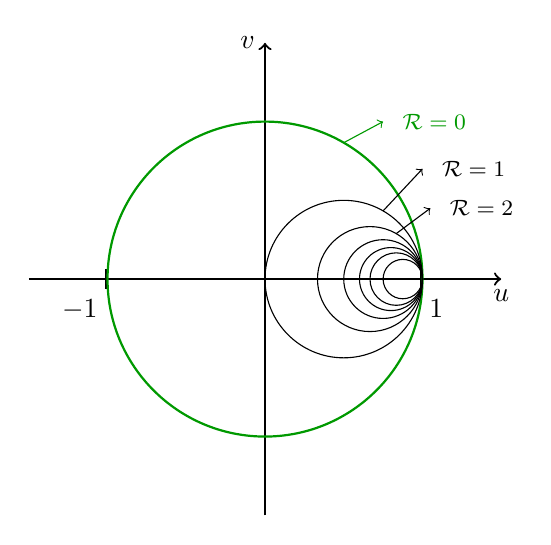
\begin{tikzpicture}
        % Axis
        \draw [thick,-|,black] (-3,0) -- (-2,0)
            node[label={below:$-1$},xshift=-1em] {};
            \draw [thick,-|,black] (-2,0) -- (2,0)
            node[label={below:$1$},xshift=0.5em] {};
        \draw[thick,->,black] (2,0)--(3,0) node[below] {$u$}; % x axis
        \draw[thick,->,black] (0,-3)--(0,3) node[left] {$v$}; % y axis
        \draw[green!60!black,thick] (0,0) circle (2);
        \draw[->,green!60!black] (1,1.732)--(1.5,2)
        node[label={[font=\footnotesize]right:$\mathcal{R}=0$}] {};
        \draw[black] (1,0) circle (1);
        \draw[->,black] (1.5,0.866)--(2,1.4)
        node[label={[font=\footnotesize]right:$\mathcal{R}=1$}] {};
        \draw[black] (4/3,0) circle (2/3);
        \draw[->,black] (2*5/6,0.866*2/3)--(2.1,0.9)
        node[label={[font=\footnotesize]right:$\mathcal{R}=2$}] {};
        \draw[black] (3*2/4,0) circle (2/4);
        \draw[black] (4*2/5,0) circle (2/5);
        \draw[black] (5*2/6,0) circle (2/6);
        \draw[black] (7*2/8,0) circle (2/8);
       \end{tikzpicture}
\end{center}\caption{Plots of different circles from the first equation}\label{fig:x_cicles} 
\end{figure}
All the circumference will collapse in $(1,0)$ when $\mathcal{R}\rightarrow\infty$\\.
For $\mathcal{R}=0$ we find the limit circumference (green one in \cref{fig:x_cicles}), this is the limit because we can not have negative real impedance.\\
Good news for the second equation in \cref{eq:normalized_impedance}, because also with this we can find some circumferences with center in $(1,\frac{1}{\mathcal{X}})$ and radius $\frac{1}{\mathcal{X}}$:
\begin{figure}[H]
    \begin{center}
        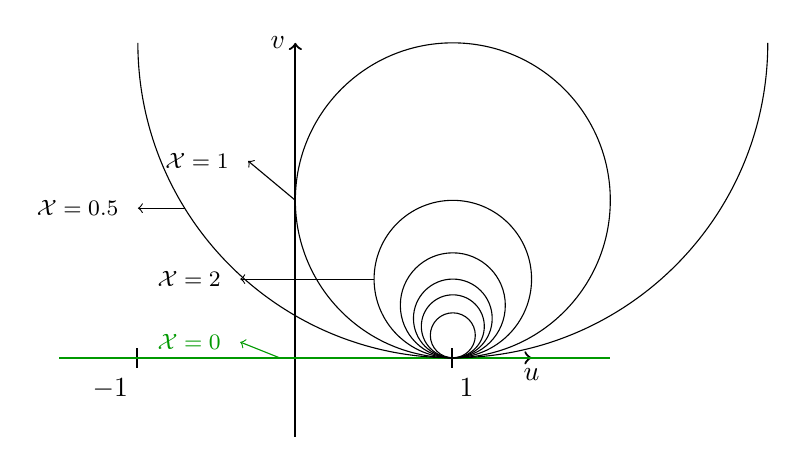
\begin{tikzpicture}
            % Axis
            \draw [thick,-|,black] (-3,0) -- (-2,0)
                node[label={below:$-1$},xshift=-1em] {};
                \draw [thick,-|,black] (-2,0) -- (2,0)
                node[label={below:$1$},xshift=0.5em] {};
            \draw[thick,->,black] (2,0)--(3,0) node[below] {$u$}; % x axis
            \draw[thick,->,black] (0,-1)--(0,4) node[left] {$v$}; % y axis
            \draw[green!60!black,thick] (-3,0) -- (4,0);
            \draw[->,green!60!black] (-0.2,0)--(-0.7,0.2)
            node[label={[font=\footnotesize]left:$\mathcal{X}=0$}] {};
            \draw[black] (2*1,2*1) circle (2*1);
            \draw[->,black] (0,2)--(-0.6,2.5)
            node[label={[font=\footnotesize]left:$\mathcal{X}=1$}] {};
            \draw[black] (2*1,2*1/2) circle (2*1/2);
            \draw[->,black] (1,1)--(-0.7,1)
            node[label={[font=\footnotesize]left:$\mathcal{X}=2$}] {};
            %\draw[black] (2*1,2*1/0.5) circle (2*1/0.5);
            \draw[->,black] (-0.35*4,1.9)--(-0.5*4,1.9)
            node[label={[font=\footnotesize]left:$\mathcal{X}=0.5$}] {};
            \draw[black] (6,2*1/0.5) arc (0:-180:2*1/0.5);
            \draw[black] (2*1,2*1/3) circle (2*1/3);
            \draw[black] (2*1,2*1/4) circle (2*1/4);
            \draw[black] (2*1,2*1/5) circle (2*1/5);
            \draw[black] (2*1,2*1/7) circle (2*1/7);
           \end{tikzpicture}
    \end{center}\caption{Plots of different circles from the second equation}\label{fig:y_cicles} 
\end{figure}
In \cref{fig:y_cicles} you can have a look at the circles made by changing the $\mathcal{R}$ parameter. When $\mathcal{R}\rightarrow \infty$ those circles collapse in $(1,0)$, then by decreasing the $\mathcal{R}$ the circumference radius will increase, until we reach the limit $\mathcal{R}=0$ where the circumference is lying in the horizontal $u$ axe (in green). You can also go in the negative part of the plot with $\mathcal{R}<0$\\
Hooray! We found a very intuitive way to represent our normalized impedance $\mathcal{Z} (l) = \mathcal{R}+j\mathcal{X}$ by choosing the right circles in my new plot that we will call \emph{Smith Chart} (Smith Will for friends). With that we can obtain the value of $v$ and $u$ of the reflection coefficient by looking at the position of the point on the plot. 
\subsubsection*{A simple example}
In this example, we want to represent $\mathcal{Z}_i = 0.2 +j0.5\si{\ohm}$ in our new plot (\cref{fig:example_plot}):
\begin{figure}[H]
    \begin{center}
        \begin{tikzpicture}
            % Axis
            \draw [thick,-|,black] (-3,0) -- (-2,0)
                node[label={below:$-1$},xshift=-1em] {};
                \draw [thick,-|,black] (-2,0) -- (2,0)
                node[label={below:$1$},xshift=0.5em] {};
            \draw[thick,->,black] (2,0)--(3,0) node[below] {$u$}; % x axis
            \draw[thick,->,black] (0,-1)--(0,4) node[left] {$v$}; % y axis
            \draw[->,black] (-0.83,1.18)--(-1.8,1.6)
            node[label={[font=\footnotesize]left:$\mathcal{Z} (l) = 0.9 +j0.5$}] {};
            \filldraw [black] (-0.83,1.18) circle (1pt);
            \draw[black] (6,2*1/0.5) arc (0:-180:2*1/0.5);
            \draw[black] (2*0.2/1.2,0) circle (2*1/1.2);
           \end{tikzpicture}
    \end{center}\caption{Smith Chart of $\mathcal{Z} (l)= 0.9 +j0.5$}\label{fig:example_plot} 
\end{figure}
By looking at the plot in \cref{fig:example_plot}, we obtain the reflection coefficient:
\begin{equation}
    \rho(l)=u+jv=|\rho| e^{\,j2\beta l}
\end{equation}
\subsubsection*{Second example}
Consider the transmission line in \cref{fig:second_example_class6} and its value of
$Z_0=50$ and $Z_L=100+j150\si{\ohm}$
\begin{figure}[H]
    \begin{center}
        \begin{circuitikz} 
            \draw (2,2)
            to[short, o-o] (7,2)
            to[short] (8.5,2)
            to[generic={$Z_{l}=140\si{\ohm}$}] (8.5,0)
            to[short, -o](7,0)
            to[short, -o](2,0)
            ;
            \draw (4.5,0.45)node[label={[font=\Large]above:$Z_0=70\si{\ohm}$}] {}
            ;
            \draw [->]  (2.5,2.3) -- (6.5,2.3)
            node[midway,yshift=0.6em]{$75\si{\centi\metre}$};
          \end{circuitikz}     
    \end{center} \caption{Transmission line of this second example}\label{fig:second_example_class6} 
\end{figure}
The first thing to do is to obtain the normalized impedance:
\begin{equation*}
    \mathcal{Z}_L=\frac{Z_L}{Z_0}=2+j3
\end{equation*}
We draw $\mathcal{Z}_L=\mathcal{Z}(l=0)$ in the Smith Chart:
\begin{figure}[H]
    \begin{center}
        \begin{tikzpicture}
            % Axis
            \draw [thick,-|,black] (-3,0) -- (-2,0)
                node[label={below:$-1$},xshift=-1em] {};
                \draw [thick,-|,black] (-2,0) -- (2,0)
                node[label={below:$1$},xshift=0.5em] {};
            \draw[thick,->,black] (2,0)--(3,0) node[below] {$u$}; % x axis
            \draw[thick,->,black] (0,-1)--(0,4) node[left] {$v$}; % y axis
            \draw[->,black] (1.2,0.4)--(-0.5,1)
            node[label={[font=\footnotesize]left:$\mathcal{Z}_L = 0.9 +j0.5$}] {};
            \filldraw [black] (1.2,0.4) circle (1pt);
            \draw[black] (2*1,2*1/2) circle (2*1/2);
            \draw[black] (3*2/4,0) circle (2/4);
           \end{tikzpicture}
    \end{center}\caption{Smith Chart of $\mathcal{Z} = 2+j3$}\label{fig:example2_plot} 
\end{figure}
Then what we can do is to look at the reflection coefficient $\rho$, not only by looking ad $u$ and $v$, but obtaining the module and the phase of the complex vector $\rho$. You can see the example in \cref{fig:example2_rho}
\begin{figure}[H]
    \begin{center}
        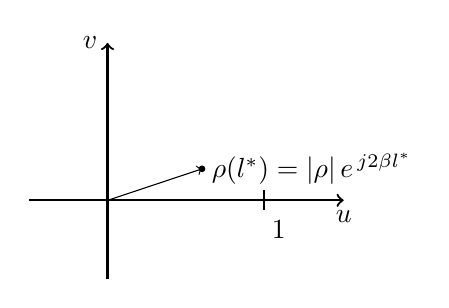
\begin{tikzpicture}
            % Axis
                \draw [thick,-|,black] (-1,0) -- (2,0)
                node[label={below:$1$},xshift=0.5em] {};
            \draw[thick,->,black] (2,0)--(3,0) node[below] {$u$}; % x axis
            \draw[thick,->,black] (0,-1)--(0,2) node[left] {$v$}; % y axis
            \filldraw [black] (1.2,0.4) circle (1pt);
            \draw[->,black] (0,0)--(1.2,0.4)node[right] {$\rho(l^*)=|\rho|\,e^{\,j2\beta l^*}$};;
           \end{tikzpicture}
    \end{center}\caption{Smith Chart of $\mathcal{Z} = 2+j3$}\label{fig:example2_rho} 
\end{figure}
According to \cref{eq:reflection_coeff_at_load2}, the module of the $\rho$ vector that we have found in the Smith chart is $\rho_L$ and it's phase angle is $2\beta l$.\\
This phase angle is very important, this is why you can find it already printed in the first outer diameter of the Smith chart, usually under the name of \emph{angle of reflection coefficient in degrees}.\\
If we move in the transmission line changing the $l$ value, in the Smith chart we will see that we are rotating the $\rho$ complex vector, but we don't change its module, like in \cref{fig:example2_rho2} 
\begin{figure}[H]
    \begin{center}
        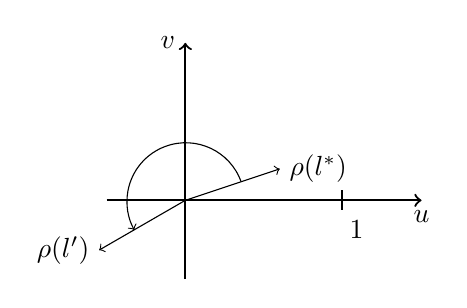
\begin{tikzpicture}
            % Axis
                \draw [thick,-|,black] (-1,0) -- (2,0)
                node[label={below:$1$},xshift=0.5em] {};
            \draw[thick,->,black] (2,0)--(3,0) node[below] {$u$}; % x axis
            \draw[thick,->,black] (0,-1)--(0,2) node[left] {$v$}; % y axis
            \draw[->,black] (0,0)--(1.2,0.4)node[right] {$\rho(l^*)$};
            \draw[black,thin, ->] (0.7071,0.24) arc (20:209:0.74672);
            \draw[->,black] (0,0)--(-1.09541,-0.6324555)node[left] {$\rho(l^\prime$)};
           \end{tikzpicture}
    \end{center}\caption{Smith Chart when we move on the line}\label{fig:example2_rho2} 
\end{figure}
We can exploit this cool behavior of the chart because whenever we move along the line, $\rho$ will rotate, and then we move in another point where we can interpolate the famous circles and we can obtain the value of the new $\mathcal{Z}$ without going troughs all the ugly formulas that we have already seen before.\\
Another interesting characteristic of this chart is that when you rotate the vector, and touch the horizontal $u$ axe, the impedance will be completely real.

If from my point i do a complete rotation, this mean that my phase variation is $2\pi$, this mean that:
\begin{align}
    \begin{split}
        &2\beta l=2\pi\\[5pt]
        2 \frac{\cancel{2\pi}}{\lambda}l&=\cancel{2\pi}\\[5pt]
    \end{split}\label{eq:phase_rotation_smith}
\end{align}
We can see in \cref{eq:phase_rotation_smith} that by completing a rotation we are moving over the line by $l=\frac{\lambda}{2}$. This is true for every rotation, so in the outer diameters of the Smith chart .\\
It is interesting to see that if we move by $l=\frac{\lambda}{4}$ we are rotating by $180\si{\degree}$, and if we look at the impedance we notice that $\mathcal{Z}_a=\frac{1}{\mathcal{Z}_b}$ as expected.\\
In the outer diameter of the Smith chart we can see also that is marked the how far we are moving from or towards the load normalized by the $\lambda$. We know also the direction because if we are moving towards the load mean that the $l$ value is increasing, and thus the angle of $\rho$, so we are moving anticlockwise in the chart.

%%--- VERY BIG SMITH CHART, TO CONTINUE TEXT SCROLL UNTIL LINE 690 ---%
\begin{figure}[H]
    \begin{center}
        \resizebox{1\textwidth}{!}{
\begin{tikzpicture}
    \pgfmathsetmacro{\xoffset}{10.45*(1-cos(3))-1.25}  
    \pgfmathsetmacro{\yoffset}{sin(3)*10.45+9.2}  
    \draw[,thick,->] (+\xoffset,\yoffset) arc [radius=10.45cm,start angle=177,end angle=166];
    \pgfmathsetmacro{\xoffset}{10.45*(1-cos(18))-1.25}  
    \pgfmathsetmacro{\yoffset}{sin(18)*10.45+9.2} 
    \draw[,draw=none] (+\xoffset,\yoffset) arc [radius=10.45cm,start angle=162,end angle=144] node[midway,sloped]{towards};
    \pgfmathsetmacro{\xoffset}{10.45*(1-cos(36))-1.25}  
    \pgfmathsetmacro{\yoffset}{sin(36)*10.45+9.2} 
    \draw[,draw=none] (+\xoffset,\yoffset) arc [radius=10.45cm,start angle=144,end angle=126] node[midway,sloped]{generator};

    \pgfmathsetmacro{\xoffset}{9.95*(1-cos(-3))-0.75}  
    \pgfmathsetmacro{\yoffset}{sin(-3)*9.95+9.2} 
    \draw[,thick,->] (\xoffset,\yoffset) arc [radius=9.95cm,start angle=183,end angle=193] ;
    \pgfmathsetmacro{\xoffset}{9.95*(1-cos(-18))-0.75}  
    \pgfmathsetmacro{\yoffset}{sin(-18)*9.95+9.2} 
    \draw[,draw=none] (+\xoffset,\yoffset) arc [radius=10.45cm,start angle=198,end angle=216] node[midway,sloped]{towards};
    \pgfmathsetmacro{\xoffset}{9.95*(1-cos(-36))-0.75}  
    \pgfmathsetmacro{\yoffset}{sin(-36)*9.95+9.2} 
    \draw[,draw=none] (+\xoffset,\yoffset) arc [radius=10.45cm,start angle=216,end angle=234] node[midway,sloped]{load};


  \begin{polaraxis}[
                    rotate=180,
                    width=23cm,
                    xshift=1.5cm, 
                    yshift=1.5cm,
                    %xticklabels={$0\lambda$,$0.05\lambda$,$0.1\lambda$,$0.15\lambda$,$0.2\lambda$,$0.25\lambda$},
                    xticklabel style={
                        sloped like x axis={%
                            execute for upside down={\tikzset{anchor=south}},
                            reset nontranslations=false
                        },
                        anchor=north,
                    },
                    xticklabel={\small\pgfmathparse{0.5-\tick/720}\pgfmathprintnumber[fixed,precision=3]{\pgfmathresult}$\lambda$},
                    xtick align=center,
                    xtick={0,18,...,360},
                    grid=none,
                    axis y line = none,
                    minor x tick num={4},
                    ymax=1,
                   ]   
 \end{polaraxis}

  \begin{polaraxis}[
                    rotate=180,
                    width=22cm,
                    xshift=1cm, 
                    yshift=1cm,
                    %xticklabels={$0\lambda$,$0.05\lambda$,$0.1\lambda$,$0.15\lambda$,$0.2\lambda$,$0.25\lambda$},
                    xticklabel style={
                        sloped like x axis={%
                            execute for upside down={\tikzset{anchor=south}},
                            reset nontranslations=false
                        },
                        anchor=north,
                    },
                    xticklabel={\small\pgfmathparse{\tick/720}\pgfmathprintnumber[fixed,precision=3]{\pgfmathresult}$\lambda$},
                    xtick align=center,
                    xtick={0,18,...,360},
                    grid=none,
                    axis y line = none,
                    minor x tick num={4},
                    ymax=1,
                   ]    

  \end{polaraxis}



  \begin{polaraxis}[
                    width=21cm,
                    xshift=-0.5cm, 
                    yshift=-0.5cm,
                    %xticklabels={$0\lambda$,$0.05\lambda$,$0.1\lambda$,$0.15\lambda$,$0.2\lambda$,$0.25\lambda$},
                    xticklabel style={
                        sloped like x axis={%
                            execute for upside down={\tikzset{anchor=north}},
                            reset nontranslations=false
                        },
                        anchor=south,
                    },
                    xticklabel={\small\pgfmathprintnumber{\tick}\si{\degree}},
                    xtick align=center,
                    grid=none,
                    axis y line = none,
                   ]    
 \end{polaraxis}

 \begin{smithchart}[
                    show origin,
                    width=20cm,
                   ]
 \end{smithchart}
 \end{tikzpicture}
    }
\end{center}\caption{Smith chart}\label{fig:beautiful_smith}
\end{figure}
%%--- very big smith chart finished ---%%



%\begin{figure}[H]
%    \begin{center}
%        \begin{tikzpicture}
%            \begin{smithchart}[
%            title=Smith Chart Stub Matching,
%            width=1\textwidth,
%            ]
%            \end{smithchart}
%        \end{tikzpicture}
%    \end{center}
%\end{figure}